\chapter{Experimental Evaluation}
\label{chapter:experimental-evaluation}
In the following chapter, we evaluate the effectiveness and the performance of the proposed ML-based partitioning advisor. We show how query featurisation affects the optimal partitioning scheme, $P^*$ (Section~\ref{sec:qfvsnonqf}) and how \citeauthor{Hilprecht:2019:TLP:3329859.3329876}'s model converges compared to the new model we develop (Section~\ref{sec:modelconv}). Additionally, we explore how the online model behaves when compound key partitioning schemes can be exploited in System-X, and build a use case for compound key partitioning schemes where it is superior (Section~\ref{sec:skvsck}). Finally, in our last evaluation (Section~\ref{sec:training-time}) we discuss the the training times required for the online phase of the RL models. 

\section{Model Definitions}
In this section, we define the terminology for the partitioning strategies we use for the rest of this chapter. 

\noindent\paragraph{RL Online.} First, we introduce the \textbf{\texttt{RL Offline}} partitioning strategy. This partitioning strategy was derived using  an offline cost model \cite{DBLP:conf/sigmod/HilprechtBR20} (which works similar to \citeauthor{DBLP:conf/sigmod/NehmeB11}'s work in \cite{DBLP:conf/sigmod/NehmeB11}). 

Automated partition designers such as \cite{DBLP:conf/sigmod/NehmeB11} usually make use of the optimiser cost estimates, i.e. they enumerate different physical designs, let the optimiser estimate the costs for all queries in the workload and choose the partitioning candidate with minimal costs. While several optimisations exist that make the integration of the optimisation and the database cost estimation tighter (e.g., \citeauthor{DBLP:conf/sigmod/NehmeB11}, \cite{DBLP:conf/sigmod/NehmeB11} make
use of the MEMO data structure in Microsoft SQL server),
they still suggest the partitioning with minimal query optimiser cost estimates. Although we would have like to test our approach against a baseline such as \cite{DBLP:conf/sigmod/NehmeB11}, System-X does not expose its query optimiser cost estimates but only its cardinality (row) estimates (Section~\ref{sec:obt-query-opt-costs}). As such, we are unable to compare \citeauthor{DBLP:conf/sigmod/NehmeB11}'s baselines against our approach.

During the offline training phase, the database partitioning is simulated and the runtimes are estimated using a network-centric cost model $c_m(P,q_i)$ approximating computation and network transfer costs of a given query $q_i$ for a partitioning strategy $P$. The cost model enumerates different join orderings similar to a query optimiser. For each individual join in the plan, it estimates the optimal join strategy and the resulting network and computation costs. The sum of the
costs is finally returned as cost estimate for the query. \citeauthor{DBLP:conf/sigmod/HilprechtBR20} show that based on this simple network-centric cost model, we can already train an DRL agent that is able to suggest reasonable partitionings. The RL Offline model can support both single and composite key partitioning strategies.

\noindent\paragraph{RL Offline + Online.} Secondly, we introduce the \textbf{\texttt{RL Offline + Online}} partitioning strategies. These partitioning strategies have been derived after refining the RL Offline models using the online phase training (Section~\ref{sec:online-training}). For the RL Offline + Online strategies, we further distinguish them between \texttt{Compound Key} and \texttt{Single Key} strategies. In \cite{DBLP:conf/sigmod/HilprechtBR20}, the online models were only trained with Single Key partitioning strategies, and such, the \texttt{RL Offline + Online} with Compound Key strategy is our first contribution towards this thesis. The single key and compound key strategies are compared in Section~\ref{sec:skvsck}. In that section, we show that the single key RL Offline + Online strategy is not suited to System-X as it does not leverage the benefits of composite key partitioning strategies. Therefore, the RL Offline Compound Key strategy is the benchmark we compare our proposed models against. Henceforth, all RL Offline strategies refer to those derived using Compound Key strategies. 

\noindent\paragraph{RL Offline + Online + Query Featurisation.} Thirdly, we introduce our second contribution - the \textbf{\texttt{RL Offline + Offline + Query Featurisation}} partitioning strategy. This strategy is derived after incorporating the query features generated using System-X's query optimiser plan + cost estimates into the DRL state model. In Section~\ref{sec:qfvsnonqf}, we show that the query-featurised partitioning performs better than our first contribution as well as the benchmark we set out to beat.

The partitioning strategies generated by all these approaches can be found in Appendix~\ref{appendix:7}.

\section{Workloads, Setups and Baselines}
For the online experiments, we use a distributed in-memory database and workloads that we explain in the following. Moreover, we discuss the learning setup that we used for training the partitioning advisors as well as the baselines we compared the DRL agent to.

\subsection{Data and Workloads}
We evaluated the partitioning advisor on the TPC-CH database schema and workloads of fixed frequencies \cite{Cole:2011:MWC:1988842.1988850}. TPC-CH is a combination of the TPC-C and TPC-H schema. The TPC-CH benchmark combines analytical queries and transactional queries in a mixed workload. For the purpose of this study, we only use the analytical queries to represent the workload in our evaluation. The TPC-CH schema has been discussed in Section~\ref{sec:tpcch}.

Similar to \cite{Hilprecht:2019:TLP:3329859.3329876, DBLP:conf/sigmod/HilprechtBR20}, we prevent co-partitioning all tables by \texttt{warehouse\_id}, since it is a trivial solution, which we do not think is suitable for many real-world schemata. Additionally, we tweak the agent so as not to use the \texttt{History, Warehouse} and \texttt{District} relations, and remove them altogether from the schema as they don't show up in any of the queries. A scale factor of 10 was used to generate the data for the online experiments, which resulted in a data size of 1 GB.

\subsection{Baselines}
\label{sec:baseline}
The baselines for the following experiments are Heuristics 1 and 2 discussed in Section~\ref{benchmarks}. These heuristics are typically used by a database administrator to physically design the data placements in the cluster.
\begin{itemize}
    \item \textbf{Heuristic 1}: greedily co-partition the largest pairs of tables while still replicating smaller tables.
    \begin{itemize}
        \item \texttt{Customer, Orders} co-partitioned using \texttt{SHARD KEY(Customer-Id)}
        \item \texttt{OrderLine, Item, Stock} co-partitioned using \texttt{SHARD KEY(Item-Id)}.
        \item \texttt{NewOrder} partitioned by \texttt{SHARD KEY(Warehouse-Id, District-Id, \\Order-Id)}        
        \item The rest of the tables are replicated.
    \end{itemize}
    \item \textbf{Heuristic 2}: naïvely replicate small tables and partitioned larger tables by primary key.
    \begin{itemize}
        \item \texttt{Customer} partitioned by \texttt{SHARD KEY(Warehouse-Id, District-Id, \\Customer-Id)}
        \item \texttt{OrderLine} partitioned by \texttt{SHARD KEY(Warehouse-Id, District-Id, \\Order-Id, Order-Number)}
        \item \texttt{NewOrder} partitioned by \texttt{SHARD KEY(Warehouse-Id, District-Id, \\Order-Id)}
        \item \texttt{Stock} partitioned by \texttt{SHARD KEY(Warehouse-Id, Item-Id)}
        \item \texttt{Orders} partitioned by \texttt{SHARD KEY(Warehouse-Id, District-Id, \\Order-Id)}
        \item The rest of the tables are replicated.
    \end{itemize}
\end{itemize}

\subsection{Learning Setup}
The partitionings were evaluated with a commercial distributed in-memory database system. We refer to this system as System-X for licensing reasons. We discuss System-X in detail in Section~\ref{sec:system-x}. System-X is particularly well suited to our online experiments because it supports composite key sharding. Additionally, owing to the utilisation of in-memory row store tables, System-X is circumvents expensive disk I/O, which results in significant reduction in query execution times and makes our learning process faster. 

For running the databases in a distributed setup, we used Amazon Web Services (AWS) cloud services. For our experiments we set up a cluster consisting of 5 nodes. Each node is located in the same availability zone inside AWS, so that latency between each node was minimal. In particular, we use 3 leaf nodes, 1 aggregator node and 1 master node. All the nodes were hosted in the \textit{ap-southeast-2} region and the \textit{average roundtrip latency} between each node was roughly $0.2$ milliseconds. Each node was allocated an instance size of \textit{r5.2xlarge}, the specifications of which are provided in Table~\ref{tab:r5.2xlarge}. The master node was allocated 100 GB of storage, and the rest of the nodes were allocated 50 GB of storage.

\begin{table}[ht]
 \centering
\begin{tabular}{|l|l|l|l|l|}
\hline
\rowcolor[HTML]{DAE8FC} 
\textbf{\begin{tabular}[c]{@{}l@{}}Instance \\ Size\end{tabular}} & \textbf{\begin{tabular}[c]{@{}l@{}}vCPU \\ count\end{tabular}} & \textbf{\begin{tabular}[c]{@{}l@{}}Memory \\ (GiB)\end{tabular}} & \textbf{\begin{tabular}[c]{@{}l@{}}Networking \\ Performance (Gbps)\end{tabular}} & \textbf{\begin{tabular}[c]{@{}l@{}}Storage \\ (GB)\end{tabular}} \\ \hline
r5.2xlarge                                                        & 8                                                              & 64                                                               & Up to 10                                                                          & 100/50                                                           \\ \hline
\end{tabular}
    \caption{r5.2xlarge specifications}
    \label{tab:r5.2xlarge}
\end{table}

\section{Limitations of System-X}
\label{sec:sysx-limitations}
In this section, we discuss some of the limitations we faced during the online phase of the training for System-X. 

\subsection{Unsupported Query Bug}
To begin with, not all queries from the TPC-CH benchmark are supported by System-X (Section~\ref{sec:penalise-query}). In order for a fair comparison between \citeauthor{Hilprecht:2019:TLP:3329859.3329876}'s model and our model, we retrained all online models with the pruned query list, which consisted of 21 queries as opposed to 22. Even then, certain partitioning schemes generated during the online phase would result in some of the queries failing due to unsupported queries in System-X. However, owing to penalising such queries with high execution times, the agent learns to avoid such partitioning schemes and produces partitioning schemes, in which all queries run perfectly. Table~\ref{tab:query-penalised} shows the percentage of total unique queries which were penalised for a unique partitioning scheme during the training phase of the query-featurised RL Online model. In addition to that limitation, System-X did not support the SQL syntax for query-13, which needed to be modified as per System-X documentation. 
\begin{table}[ht]
 \centering
\begin{tabular}{|rr|}
\hline
\multicolumn{1}{|l|}{\textbf{\# unique queries ran}} & \multicolumn{1}{l|}{\textbf{\# unique queries failed}} \\ \hline
\multicolumn{1}{|r|}{3549}                           & 7                                                      \\ \hhline{|=|=|}
\textbf{\% of queries penalised}                     & \textbf{0.20}                                          \\ \hline
\end{tabular}
    \caption{Percentage of queries penalised with respect to unique partitioning schemes.}
    \label{tab:query-penalised}
\end{table}

As an aside, after communicating the issue to System-X engineers, the unsupported query was confirmed to be a bug, which occurred due to an query optimisation operation in System-X. Owing to the agent exploring multiple partitioning schemes, we were able to identify certain partitionings where individual queries would not work owing to the specific partitioning. After this discovery, the System-X engineers have identified the bug, and will be shipping a patch in the next version. 

\subsection{Dynamic Repartitioning}
A major challenge was the dynamic repartitioning problem in System-X. By default, System-X does not support dynamic repartitioning out of the box, which is why we needed to perform the repartitioning in a roundabout manner. Compare the following syntax, where Listing~\ref{listing:pgsql-partitioning} is the equivalent query in PostgresXL to Listing~\ref{listing:systemx-partitioning} in System-X. 

\begin{listing}[ht]
\inputminted[frame=lines,
            breaklines=true,
            framesep=2mm,
            fontsize=\footnotesize]
            {sql}
            {listings/pgxl-partitioning.sql}
\caption{Example code to repartition by Hash Key in PostgresXL.}
\label{listing:pgsql-partitioning}
\end{listing}

\begin{listing}[ht]
\inputminted[frame=lines,
            breaklines=true,
            framesep=2mm,
            fontsize=\footnotesize]
            {sql}
            {listings/sysx-partitioning.sql}
\caption{Example code to repartition by Shard Key in System-X.}
\label{listing:systemx-partitioning}
\end{listing}

This step means that a lot of custom code is required to produce the desired partitioning scheme the agent chooses for a particular schema. This is because the repartitioning step requires us to physically code the schema of the database (in this case the TPC-CH schema) and recreate the indexes on the tables. However, in future versions of System-X, this issue will not persist as dynamic partitioning syntax will be supported. 

\section{Single Key vs Compound Key Partitioning}
\label{sec:skvsck}

With the first experiment we aim to quantify the benefits of supporting compound key partitioning strategies in the learning advisor. We compare the results of using single-key partitioning strategies developed by \citeauthor{Hilprecht:2019:TLP:3329859.3329876} to the performance of our compound-key enhanced learning advisor. 
The comparison of query runtimes of both models on the TPC-CH database after running the query workload 100 times are shown in Figure~\ref{fig:skvsck}.

\begin{figure}[hb]
  \centering
  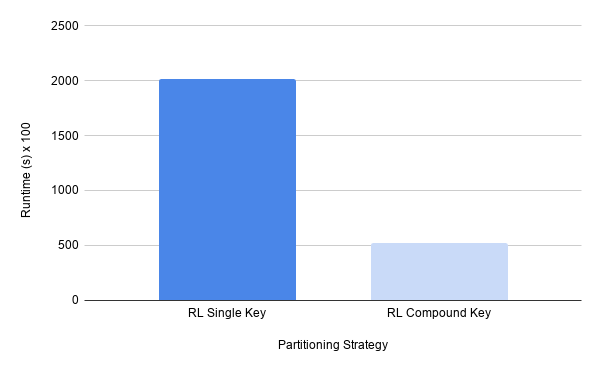
\includegraphics[width=\linewidth]{figures/skvsck-query-runtimes.png}
  \mycaption{Query execution time of query workloads with single key and compound key models}{In this figure, we show that the partitioning scheme suggested by the online phase of the non-query featurised and compound key RL model is far superior to that of the RL model which only relies on single keys for sharding. On average, the query execution time has a \textbf{4x speedup} with RL Compound Key partitioning over RL Single Key partitioning.}
  \label{fig:skvsck}
\end{figure}

Both models are first trained offline, and then refined in an online training phase. Each online model is trained on the TPC-CH benchmark with a scaling factor, $SF=10$, and for the workloads we assumed that all queries occur equally frequently. To be more elaborate, these query execution times are measured after running the TPC-CH query workload 100 times on each partitioning scheme and then by measuring the total time taken for each run to complete. The queries are run 100 times over to average across small discrepancies in the query execution time which occur frequently over time due to random chance, e.g. network latency and hardware performance. By running the queries multiple times, we show that the query execution times differ not only by chance, but mainly due to our dependent variables - which are the partitioning schemes for each relation. 

As shown later in Figure~\ref{fig:query-runtimes}, even standard heuristics, which co-partition relations using compound keys perform better single key co-partitioning schemes simply because of the TPC-CH query workload executing faster in compound key partitioning strategies due to better co-partitioning of tables. In the case of System-X, our compound key agent massively outperforms the single key agent - by providing a \textbf{4x speedup}. The single-key partitioning model suggests the following partition: \texttt{NewOrder}, \texttt{Order}, and \texttt{Orderline} tables are co-partitioned by \texttt{Order-Id} and the rest of the tables are replicated. The compound-key online advisor (\textit{without query-featurisation}) on the other hand suggests the following partition: \texttt{NewOrder}, \texttt{Order}, \texttt{Orderline} and \texttt{Customer} tables are co-partitioned by \texttt{(Warehouse-Id, District-Id)}; the \texttt{Supplier} table is partitioned by the \texttt{Supplier-Key}, and the rest are replicated. 


% Physical Design Strategy instead of Partitioning Strategy
\section{Query Featurisation vs Non-Featurisation}
\label{sec:qfvsnonqf}
In our second experiment, we evaluate whether the query-featurised version of the DRL advisor finds partitions that are better than its non-query-featurised counterparts. Additionally, we show that both our online models perform better than the RL Offline model developed by \citeauthor{Hilprecht:2019:TLP:3329859.3329876}. To recap, the RL Offline model suggests the following partitioning scheme: \texttt{NewOrder}, \texttt{Order}, \texttt{Orderline} and \texttt{Customer} tables are co-partitioned by \texttt{(Warehouse-Id, District-Id)}; the \texttt{Stock} and \texttt{Supplier} tables are co-partitioned by the \texttt{Supplier-Key}, and the rest are replicated. 

Here, we first train the offline models for System-X, and then refine one model with query-featurisation online training, and another without. For a fair comparison, we train both online models with compound key partitioning strategies. Each online model is trained on the TPC-CH benchmark with a scaling factor, $SF=10$, and for the workloads we assumed that all queries occur equally frequently. To demonstrate that our model is superior to its predecessors, we compare our model against the non-query featurised version of the model, the offline model and the Heuristics 1 and~2. The results of using the best partitioning found by each model on the TPC-CH database are shown in Figure~\ref{fig:query-runtimes} after running the query workload 100 times on partitioning schemes suggested by each model and heuristic. 

Firstly, the RL Offline + Online model improves on the RL Offline model by identifying that replicating the \texttt{Supplier} table produces better results than co-partitioning it with \texttt{Stock}. Secondly, the query-featurised model improves on the non-featurised version by suggesting the following partitioning scheme: \texttt{Customer} partitioned by \texttt{(District-Id, Warehouse-Id)}, \texttt{Order, NewOrder} and \texttt{OrderLine} co-partitioned by \texttt{(Order-Id, District-Id, Warehouse-Id)}, \texttt{Nation} and \texttt{Region} co-partitioned by \texttt{Region-Key}, \texttt{Stock} and \texttt{Supplier} co-partitioned by the \texttt{Supplier-Key}, while the rest are replicated. The interesting result here is that the query-featurised model is capable of identifying sharding keys which are compound aggregations made up of \textbf{three} attributes - which shows that the model is capable of recognising and exploiting the fact that only three relations could be co-partitioned by the \texttt{(Order-Id, District-Id, Warehouse-Id)} compound key.

% Make sure that the captions are a bit more self-explanatory

\begin{figure}[H]
  \centering
  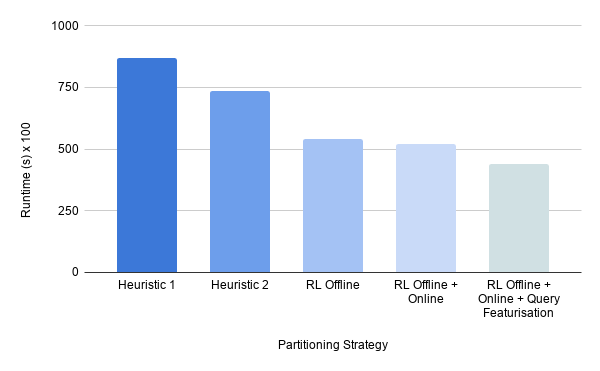
\includegraphics[width=\linewidth]{figures/query-runtimes.png}
  \vspace*{-1.5\baselineskip}
  \mycaption{Query execution times of query workload in different partitionings proposed by the DRL agent and heuristics}{In this figure, we show our primary contributions towards creating better learners with the RL Offline + Online and RL Offline + Online + Query Featurisation models. Both of our proposed models beat the benchmark, RL Offline for System-X, by incrementally producing speedups of \textbf{1.03x} and \textbf{1.23x} on the TPC-CH query workload. The actual runtimes can be found in Appendix~\ref{appendix:3}.\vspace{-0.5\baselineskip}}
  \label{fig:query-runtimes}
\end{figure}

Similar to Figure~\ref{fig:skvsck}, in this experiment, we run the query workload across each partitioning scheme 100 times in order to average the effect of random variables, e.g. network latency and hardware performance. This figure demonstrates the core contribution of our work. All the online models trained on System-X outperform the heuristics as well as the RL Offline model - the benchmark which we are trying to beat. As expected, the RL Offline + Online model outperforms just the RL Offline model, by refining the partitioning found by the RL Offline model. Additionally, we improve on the RL Offline + Online model by proposing query-featurisation as part of modelling the state in the DRL agent. As such, we contribute two optimisations to the existing DRL agent proposed by \citeauthor{Hilprecht:2019:TLP:3329859.3329876} and show that our optimisations provide incremental speedups of \textbf{1.03x} and \textbf{1.23x} compared to the RL Offline model for the RL Offline + Online and RL Offline + Online + Query Featurisation models respectively.

\subsection{Benefits of Query Featurisation}
\label{sec:benefits-query-featurisation}
As we covered already, the query-featurised online model is capable of finding partitioning schemes, where the query execution times are faster than those of its counterparts. After some thorough inspection using System-X's query-profiler, we can investigate why the partitioning scheme produced by the query-featurised model performs better. For this experiment, we execute the query workload multiple times on each of the best partitioning schemes found by the RL Offline, RL Offline + Online and the RL Offline + Online + Query Featurisation models, and then calculate the average network traffic and memory usage costs for each partitioning. The results are shown in Figure~\ref{fig:network-memory}. 

\begin{figure}
     \centering
     \begin{subfigure}[b]{.9\textwidth}
          \centering
          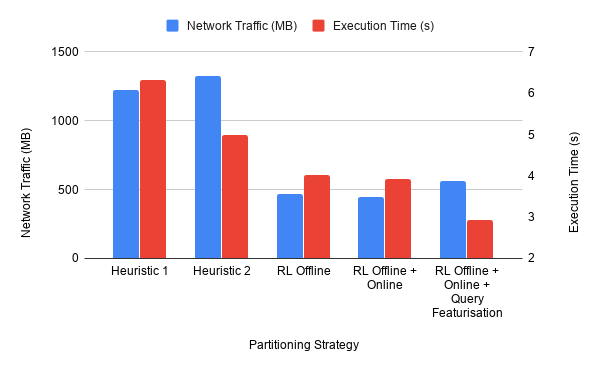
\includegraphics[width=1\linewidth]{figures/network-traffic.png}
          \caption{Average Network Traffic (MB) for TPC-CH query workload on System-X.}
          \label{fig:network-traffic}
     \end{subfigure}
     \hfill
     \begin{subfigure}[b]{.9\textwidth}
          \centering
          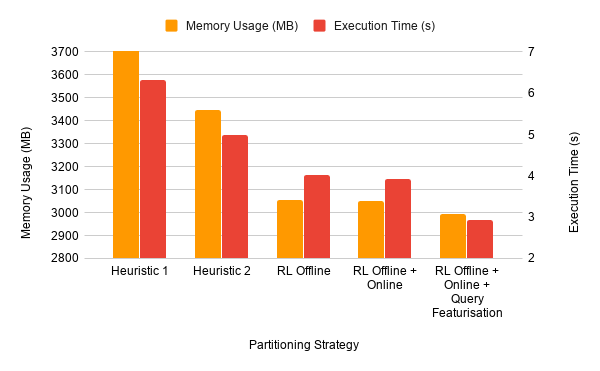
\includegraphics[width=1\linewidth]{figures/memory-usage.png}
          \caption{Average Memory Usage (MB) for TPC-CH query workload on System-X.}
          \label{fig:memory-usage}
     \end{subfigure}
     \mycaption{Average network traffic and memory usage across RL partitioning schemes and heuristics}{This figure shows that lower memory usage appears to have a bigger impact in terms of query execution time than network traffic does. Heuristic 1 actually has a massive memory usage of 15 GB, which cannot be viewed in this graph. As stated previously, with networking performance of up to 10 Gbps in our AWS cluster, memory usage appears to dominate the effects of network traffic. Therefore, it appears that the query-featurised RL model prefers to prioritise query-workload states (\textit{features}), which reduce memory usage, i.e faster joins, but increase network traffic, i.e. higher repartition and broadcast costs. The actual memory usage and network traffic have been displayed in Appendix~\ref{appendix:4}.}
     \label{fig:network-memory}
\end{figure}

This experiment relays a key finding in support of the Query Featuriser. While the RL Offline + Online partitioning did perform better than the RL Offline partitioning in terms of reducing the total network traffic and memory usage for each query and also had lower network traffic compared to the Query-Featurised partitioning, it still executed the queries slower than the Query-Featurised partitioning because of significantly higher memory usage. The featurised costs from the query optimiser for the TPC-CH query workload aided the query-featurised model to find optimal partitioining schemes which favoured lower memory usage over higher network traffic. Although not very intuitive, memory usage appears to play a bigger role in terms of reducing query execution time than network traffic does, as we observed from the query execution runtimes in Figure~\ref{fig:query-runtimes} for System-X and our given experimental setup. Owing to the black box nature of Deep Neural Networks, it is difficult to ascertain how query featurisation enables better partitioning schemes from the model itself. As such, our final investigation into Network Traffic and Memory Usage provides an indicator to show case that the normalised query features consisting of Join costs (\textit{Memory Usage}); and Repartitioning and Broadcast costs (\textit{Network Traffic}) show us that the query-featurised model learns to activate the maximum reward actions to reach the optimal query-feature states encoding optimal network traffic and memory usage after each time step of the training phase. A similar argument can be made for why Heuristic-2 has faster query execution times than Heuristic-1, i.e. owing to lower memory usage and higher network traffic. It is fascinating to note, however, that the query-featurised RL Model was capable of finding a balance between network traffic and memory usage to enable the fastest query runtimes.

\section{DRL Convergence}
\label{sec:modelconv}
In our next experiment, we show that the query-featurised agent performs \textit{as good, or better} in terms of finding the optimal 
partitioning schemes than the non-query-featurised agent. For this experiment, we train the online models up to 2000 episodes, and extract the best solutions periodically every 100 episodes. Then, for each solution produced by each model, we measure the runtimes by running the TPC-CH query workload 10 times across each partitioning scheme produced periodically across every 100 episodes. The runtimes are shown in Figure~\ref{fig:model-convergence}.

The results show that the query featurised version finds the optimal partitioning scheme within 1000 episodes, whereas the non-featurised version finds its optimal partitioning scheme within 1500 episodes. The models then oscillate around their optimal partitioning schemes after further training. These results show that the query-featurised scheme not only finds better partitioning schemes, but also finds them quicker than the non-query-featurised version.


\begin{figure}[h]
  \centering
  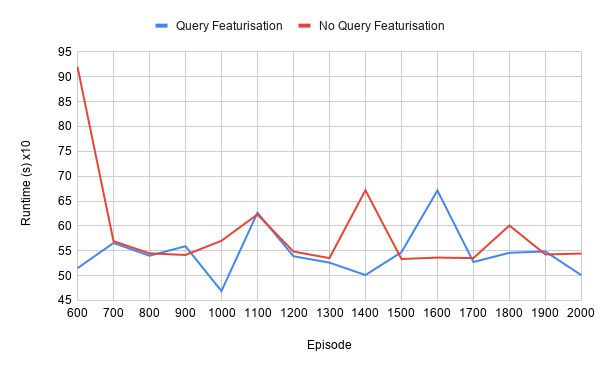
\includegraphics[width=\linewidth]{figures/model-convergence.png}
  \caption{Query execution time across episodes for query-featurised and non-featurised RL Models.}
  \label{fig:model-convergence}
\end{figure}

\subsection{Limitations of the Online Phase}
\label{sec:limitations-of-online-phase}
The best models across each episode show that the RL Online models are not ideally precise about recording the lowest rewards. This is primarily due to hardware and network imprecision during training the online model. The online training phase uses the minimum of two runtimes of each query for every unique partitioning state combination. However, owing to network and hardware imprecision, sometimes the actual runtimes of the queries might not reflect the optimal runtime if all network and hardware conditions were assumed to be ideal. As such, as seen from Figure~\ref{fig:model-convergence}, although the query featurised model finds a better partitioning scheme in episode 1000, it reaches very similar solutions in episodes 1400 and 2000, but not as good. 

\section{Training Time}
\label{sec:training-time}
In our final experiment, we discuss the total training time with respect to our current workload baselines and training hyperparameters. The training time of a reinforcement learning agent can be determined by two factors - the $\epsilon$ and the $\epsilon\textit{-decay}$ values. Given our starting value of $\epsilon = 1$  and $\epsilon\textit{-decay} = 0.997$, our models are expected to exploit maximum reward actions with a $99\%$ probability and only explore actions randomly at $1\%$ probability when the $\epsilon$ value reaches $0.01$ (i.e. exploration rate of $1\%$) after $\approx 1560$ episodes. Traditionally, RL agents are trained until a minimum value of $\epsilon = 0.01$ is reached. However, for our case, we empirically decide on training the agent for 1200 episodes, at which point $\epsilon = 0.027$ in order to minimise training time, and because the RL partitioning schemes after 1200 episodes are already better than the RL Offline partitioning benchmark. The total training times along with the total repartitioning time for the online models are shown in Table~\ref{tab:training-time}.
\begin{table}[ht]
 \centering
\begin{tabular}{|l|r|r|r|}
\hline
\rowcolor[HTML]{DAE8FC} 
\cellcolor[HTML]{DAE8FC}\textbf{RL Model}                                           & \multicolumn{1}{l|}{\cellcolor[HTML]{DAE8FC}\textbf{\begin{tabular}[c]{@{}l@{}}Total Training\\ Time (s)\end{tabular}}} & \multicolumn{1}{l|}{\cellcolor[HTML]{DAE8FC}\textbf{\begin{tabular}[c]{@{}l@{}}Total Repart-\\ ioning Time (s)\end{tabular}}} & \multicolumn{1}{l|}{\cellcolor[HTML]{DAE8FC}\textbf{\begin{tabular}[c]{@{}l@{}}\% Repartitioning \\ time\end{tabular}}} \\ \hline
RL Online + Offline                                                                 & 48612                                                                                                                   & 15542                                                                                                                         & 32.0                                                                                                                    \\ \hline
\begin{tabular}[c]{@{}l@{}}RL Online + Offline\\ + Query Featurisation\end{tabular} & 52177                                                                                                                   & 15957                                                                                                                         & 30.6                                                                                                                    \\ \hline
\end{tabular}
    \mycaption{Training time for RL Online models in System X}{The query-featurised RL model finds the best solution around 1000 episodes, and the non query-featurised one finds its best solution around 1500 episodes. The actual values for the model training times can be found in Appendix~\ref{appendix:5}.}
    \label{tab:training-time}
\end{table}

\subsection{Discussion of Training Time}
\label{sec:discussion-training-time}
As stated in Table~\ref{tab:training-time}, a majority of the training time is dominated by the total repartitioning time required after the agent repartitions or replicates tables. Generally, this would not be an issue, but as discussed in Section~\ref{sec:sysx-limitations}, System-X is not well suited to dynamic repartitioning since it is not a supported operation. As such, our custom repartitioning scripts which rely on duplication of data followed by deletion of data is not only time-consuming, but a memory-intensive operation as well. Since System-X is an in memory database, this roundabout way of repartitioning involves massive memory-usage, which can often result in System-X leaves running out of memory during a repartitioning operation - particularly during the deletion of large tables. In summary, this unoptimised repartitioning strategy results in long repartitioning times, which significantly increases the training time.
However, in terms of practical applications for our model, we believe that a training time of several hours is acceptable since the model only has to be trained once, after which the Query Runtime Caches and Query Feature Cost Caches can be reused to re-train other models. Moreover, especially in cloud setups, we can easily clone the instances. Hence, setting up a similar cluster to retrain the agent for several hours to obtain a refined model should be feasible considering that customers usually have one cluster provisioned all the time to do analytics.

\section{Discussions and Limitations of our Evaluation}
\label{sec:discussion-limitation-evaluation}
Although we have seen substantial improvements in query runtime execution as well as model convergence within a fewer number of episodes, we would wish to explore the following experiments in order to substantially verify its usability and performance.

\subsection{Query Execution Evaluation}
For our experiments to showcase the differences between the the different partitionings proposed by the RL models and heuristics, we choose to run the query workload 100 times over. While 100 appears to be an arbitrary number, we essentially take this step in order to simulate the extension of the workload in order to get a reasonable duration for the performance of the experiments of about an hour or so. 100 is indeed an exhaustive number, but owing to the variation of the individual query runtimes we experienced in the AWS cluster, and due to the fact that each query is executed very quickly in an in-memory database, we empirically use 100 runs as a baseline to measure the performances of each partitioning scheme.

\subsection{Adaptivity to workload mixes}
Currently, all our experiments assume uniform frequency of query workloads across each timestep of the RL training phase. In order to remedy this uniformity, we would need to alter the workload frequency state vector from Equation~\ref{eq:workload-frequency}. This can be quite easily done by introducing different workload mixes, and then evaluating the performance through query execution runtimes. 

\subsection{Adaptivity to hardware deployment}
All our experiments are currently hosted in AWS cloud instances, where all the instances have the same hardware specifications, and the network latency between the cluster instances also remain fixed. It would be ideal to measure runtimes across varying hardware specifications and network conditions in order to assess the effectiveness of our models. This could be achieved by specifying different instance sizes for our cluster nodes, and deploying the nodes across different availability zones in order to vary the latency across nodes. This would enable us to study the generalisability of our model across various hardware deployments for more practical use cases.  

\subsection{Adaptivity to dynamic query workloads}
In all of our experiments previously, we have only worked with static query workloads - which is not ideal in practical applications. For dynamic query workloads, one solution is to simply retrain the neural network with a different set of queries, which would enable the RL agent to adapt to the new set of queries. This step could be imagined as being analogous to refining the offline phase model with the online training. 
However, in our proposed query-featurised model, the query optimiser adapting to dynamic queries adds an added level of complexity towards the state representation of the queries. In general, the query plan representation in the state is already more generic than the standard query text, as the database query optimiser will perform some internal translation to a generic form of a query and optimise that. So, vastly different SQL query formulation might end up with the same internal plan, which is good for keeping the state small and generic at the same time.
However, query selectivity plays an important role into this as query optimiser cardinality estimates will vary due to differences in queries, e.g. filter predicates. Currently, we only assume that a known workload is generated by an application with a fixed number of queries, and we capture the most common executions. If the queries have similar selectivites, they will be covered. If they differ vastly, or if they are ad-hoc queries, we currently do not support them and the work required to do so are beyond the scope of this thesis. 

% Talk about incremental imrpovements from single --> compound --> query featurised and show speedups
% Show network costs/repartitioning/broadcast cost changes across each optimal partition suggested by each agent.

% Talk about how long it takes, and how RL is slow 
% Training time for each 
% How general it is to other databases
% Talk about how long it takes to partition vs total training time -- % WHy did you fix it? 
% What happens if you don't fix it?
% Why 100 times and not 200 times?
